\chapter{Surface Facility}
\label{ch:fscf-surf-facil}

%%%%%%%%%%%%%%%%%%%%%%%%%%%%%%%%%%%%%%%%%%%%%%%%%%%%%%%%%%%%%%%%%%%
\section{Existing Surface Facility}
\label{sec:fscf-surf-facil-existing}


The Sanford Laboratory property of 186 acres consists of steep terrain and man-made cuts dating from its mining history. There are approximately 50 buildings and associated site infrastructure in various states of repair. A select few of these buildings at the Ross Complex and the main utilities are needed by the LBNF experiment and will be upgraded and rehabilitated as necessary. A layout of the overall Sanford Laboratory architectural site plan for the LBNF Project is found in Figure~\ref{fig:archit-site-plan}.
The Ross Complex will house the facility construction operations, command and control center for the experiment and facility, new cryogenics compressor building, as well as continue to house the Sanford Laboratory maintenance and operations functions. Layout of surface facilities in the vicinity of the Ross Shaft is shown in Figure~\ref{fig:ross-archit-site-plan}.

\begin{cdrfigure}[Architectural site plan]{archit-site-plan}{Architectural site plan (HDR)}
%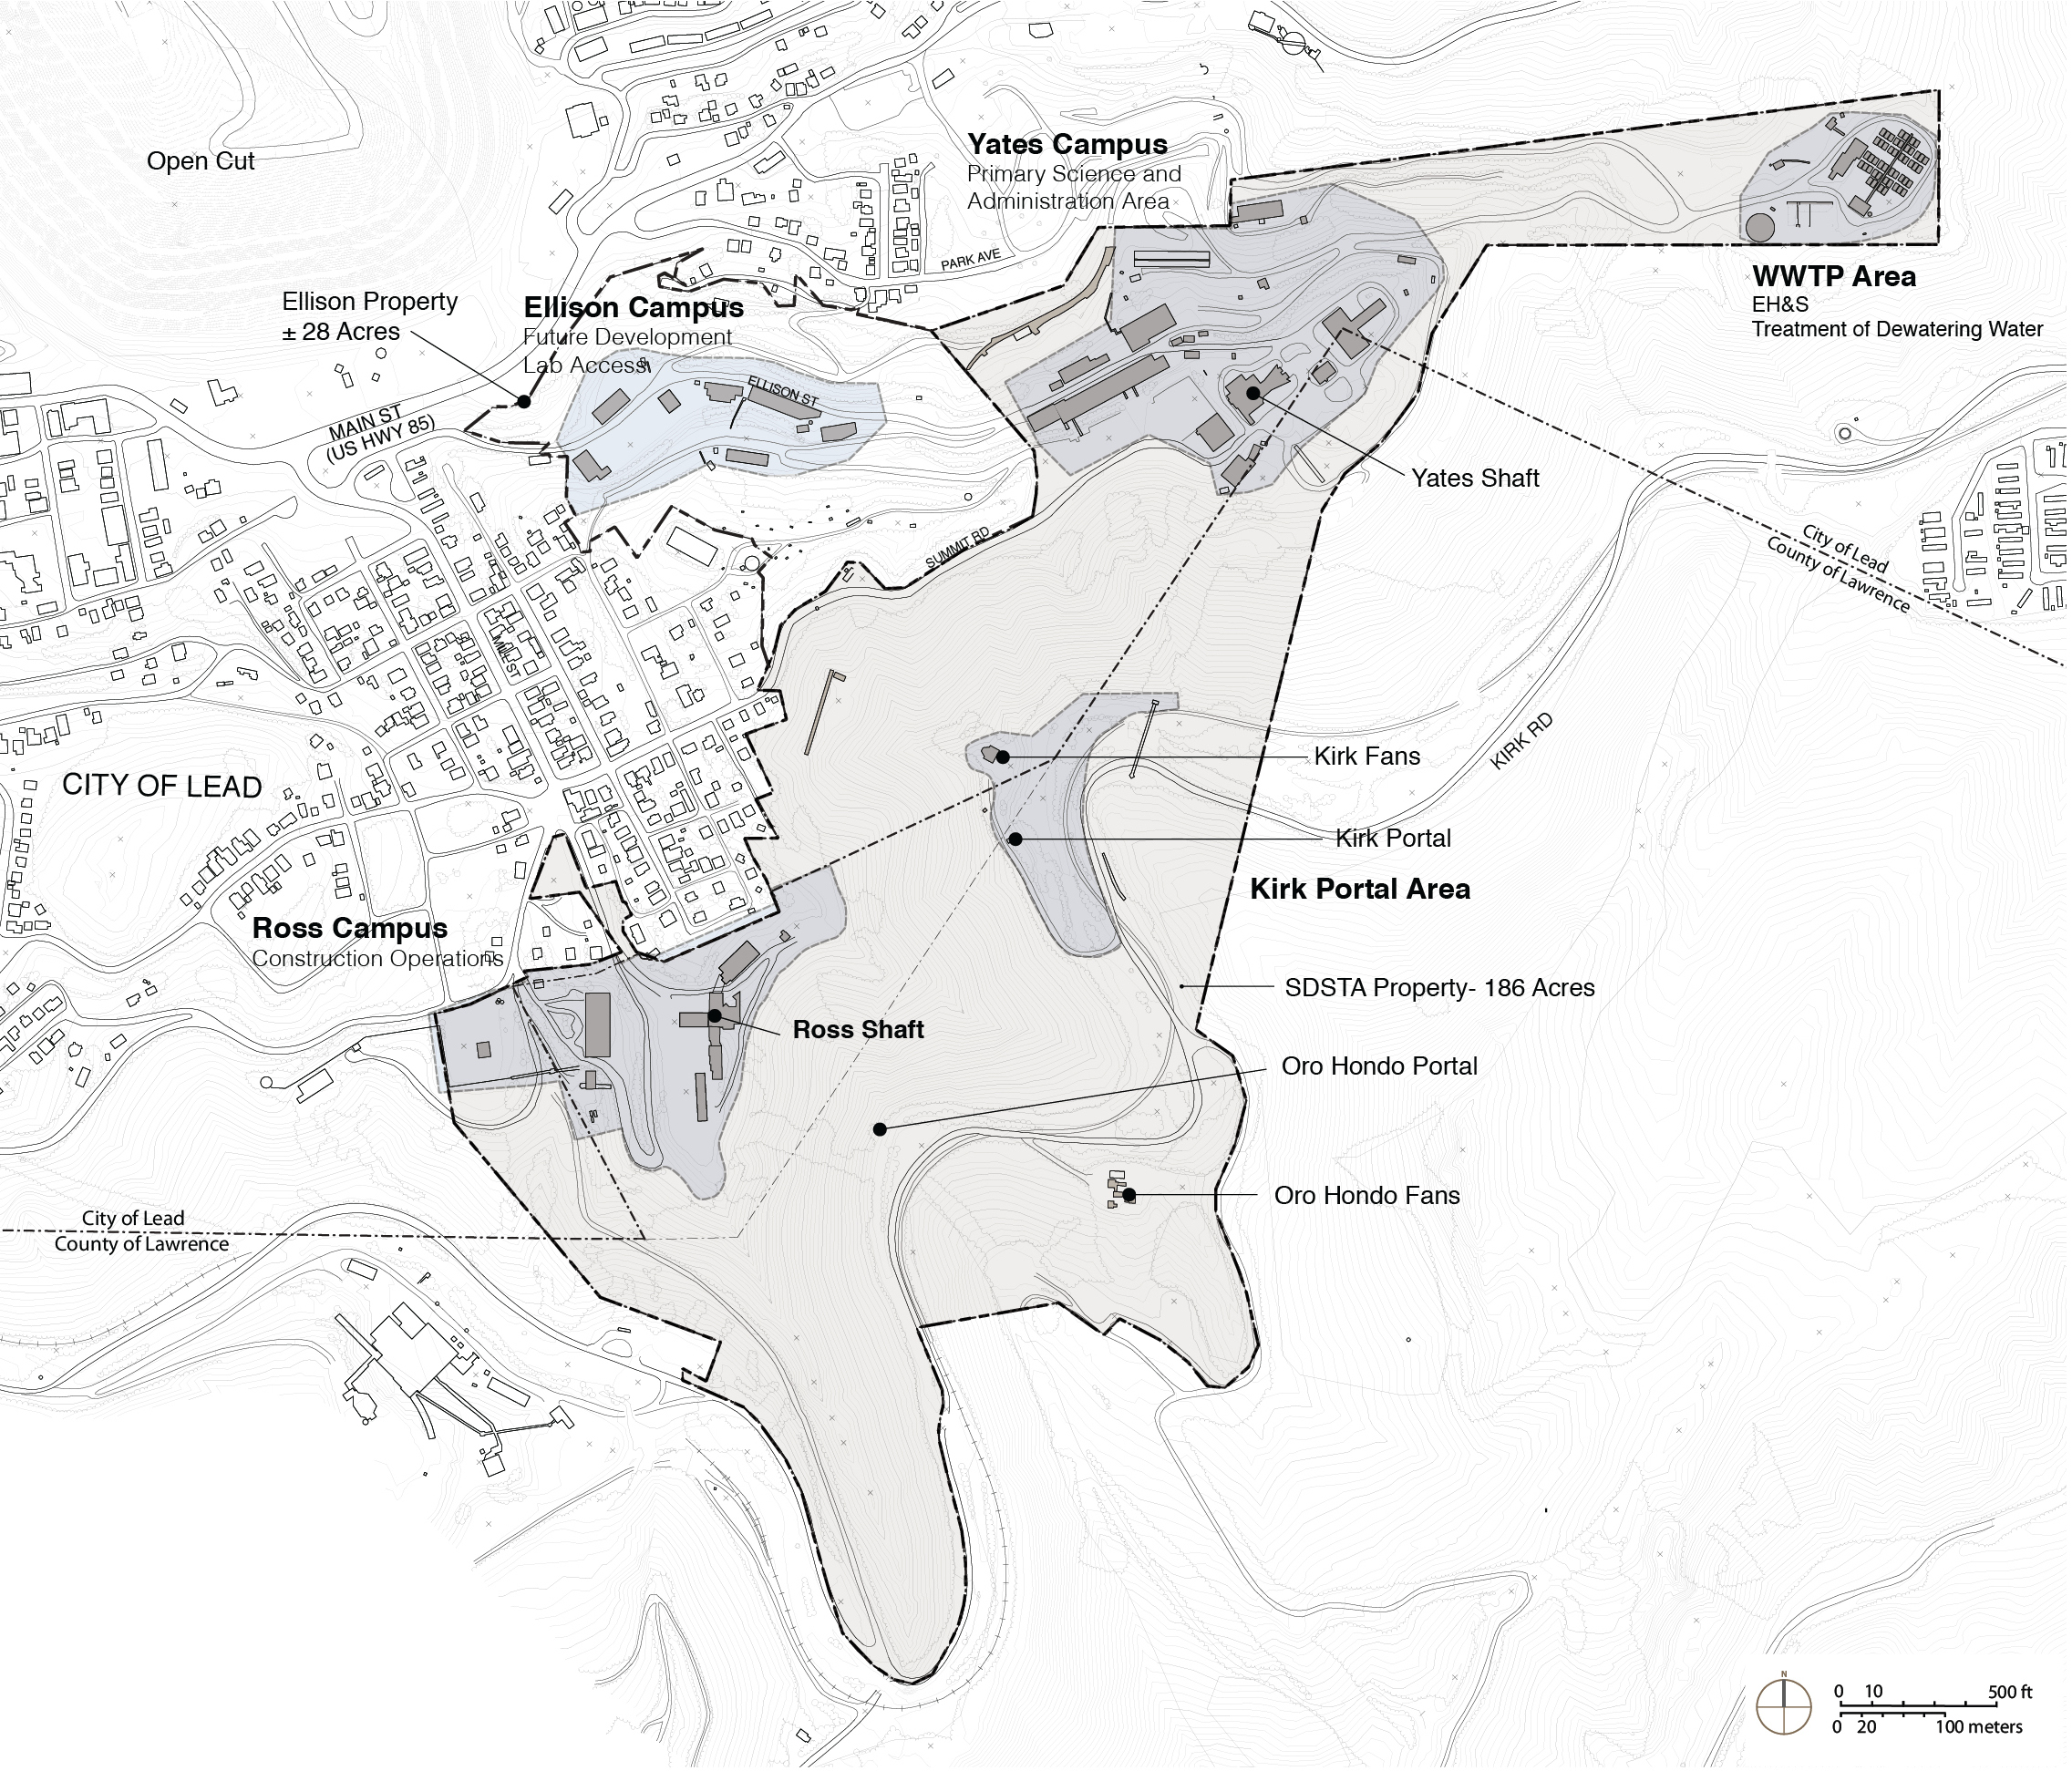
\includegraphics[width=0.8\textwidth]{archit-site-plan}
\end{cdrfigure}

\begin{cdrfigure}[Ross Complex architectural site plan]{ross-archit-site-plan}{Ross Complex architectural site plan (Arup)}
%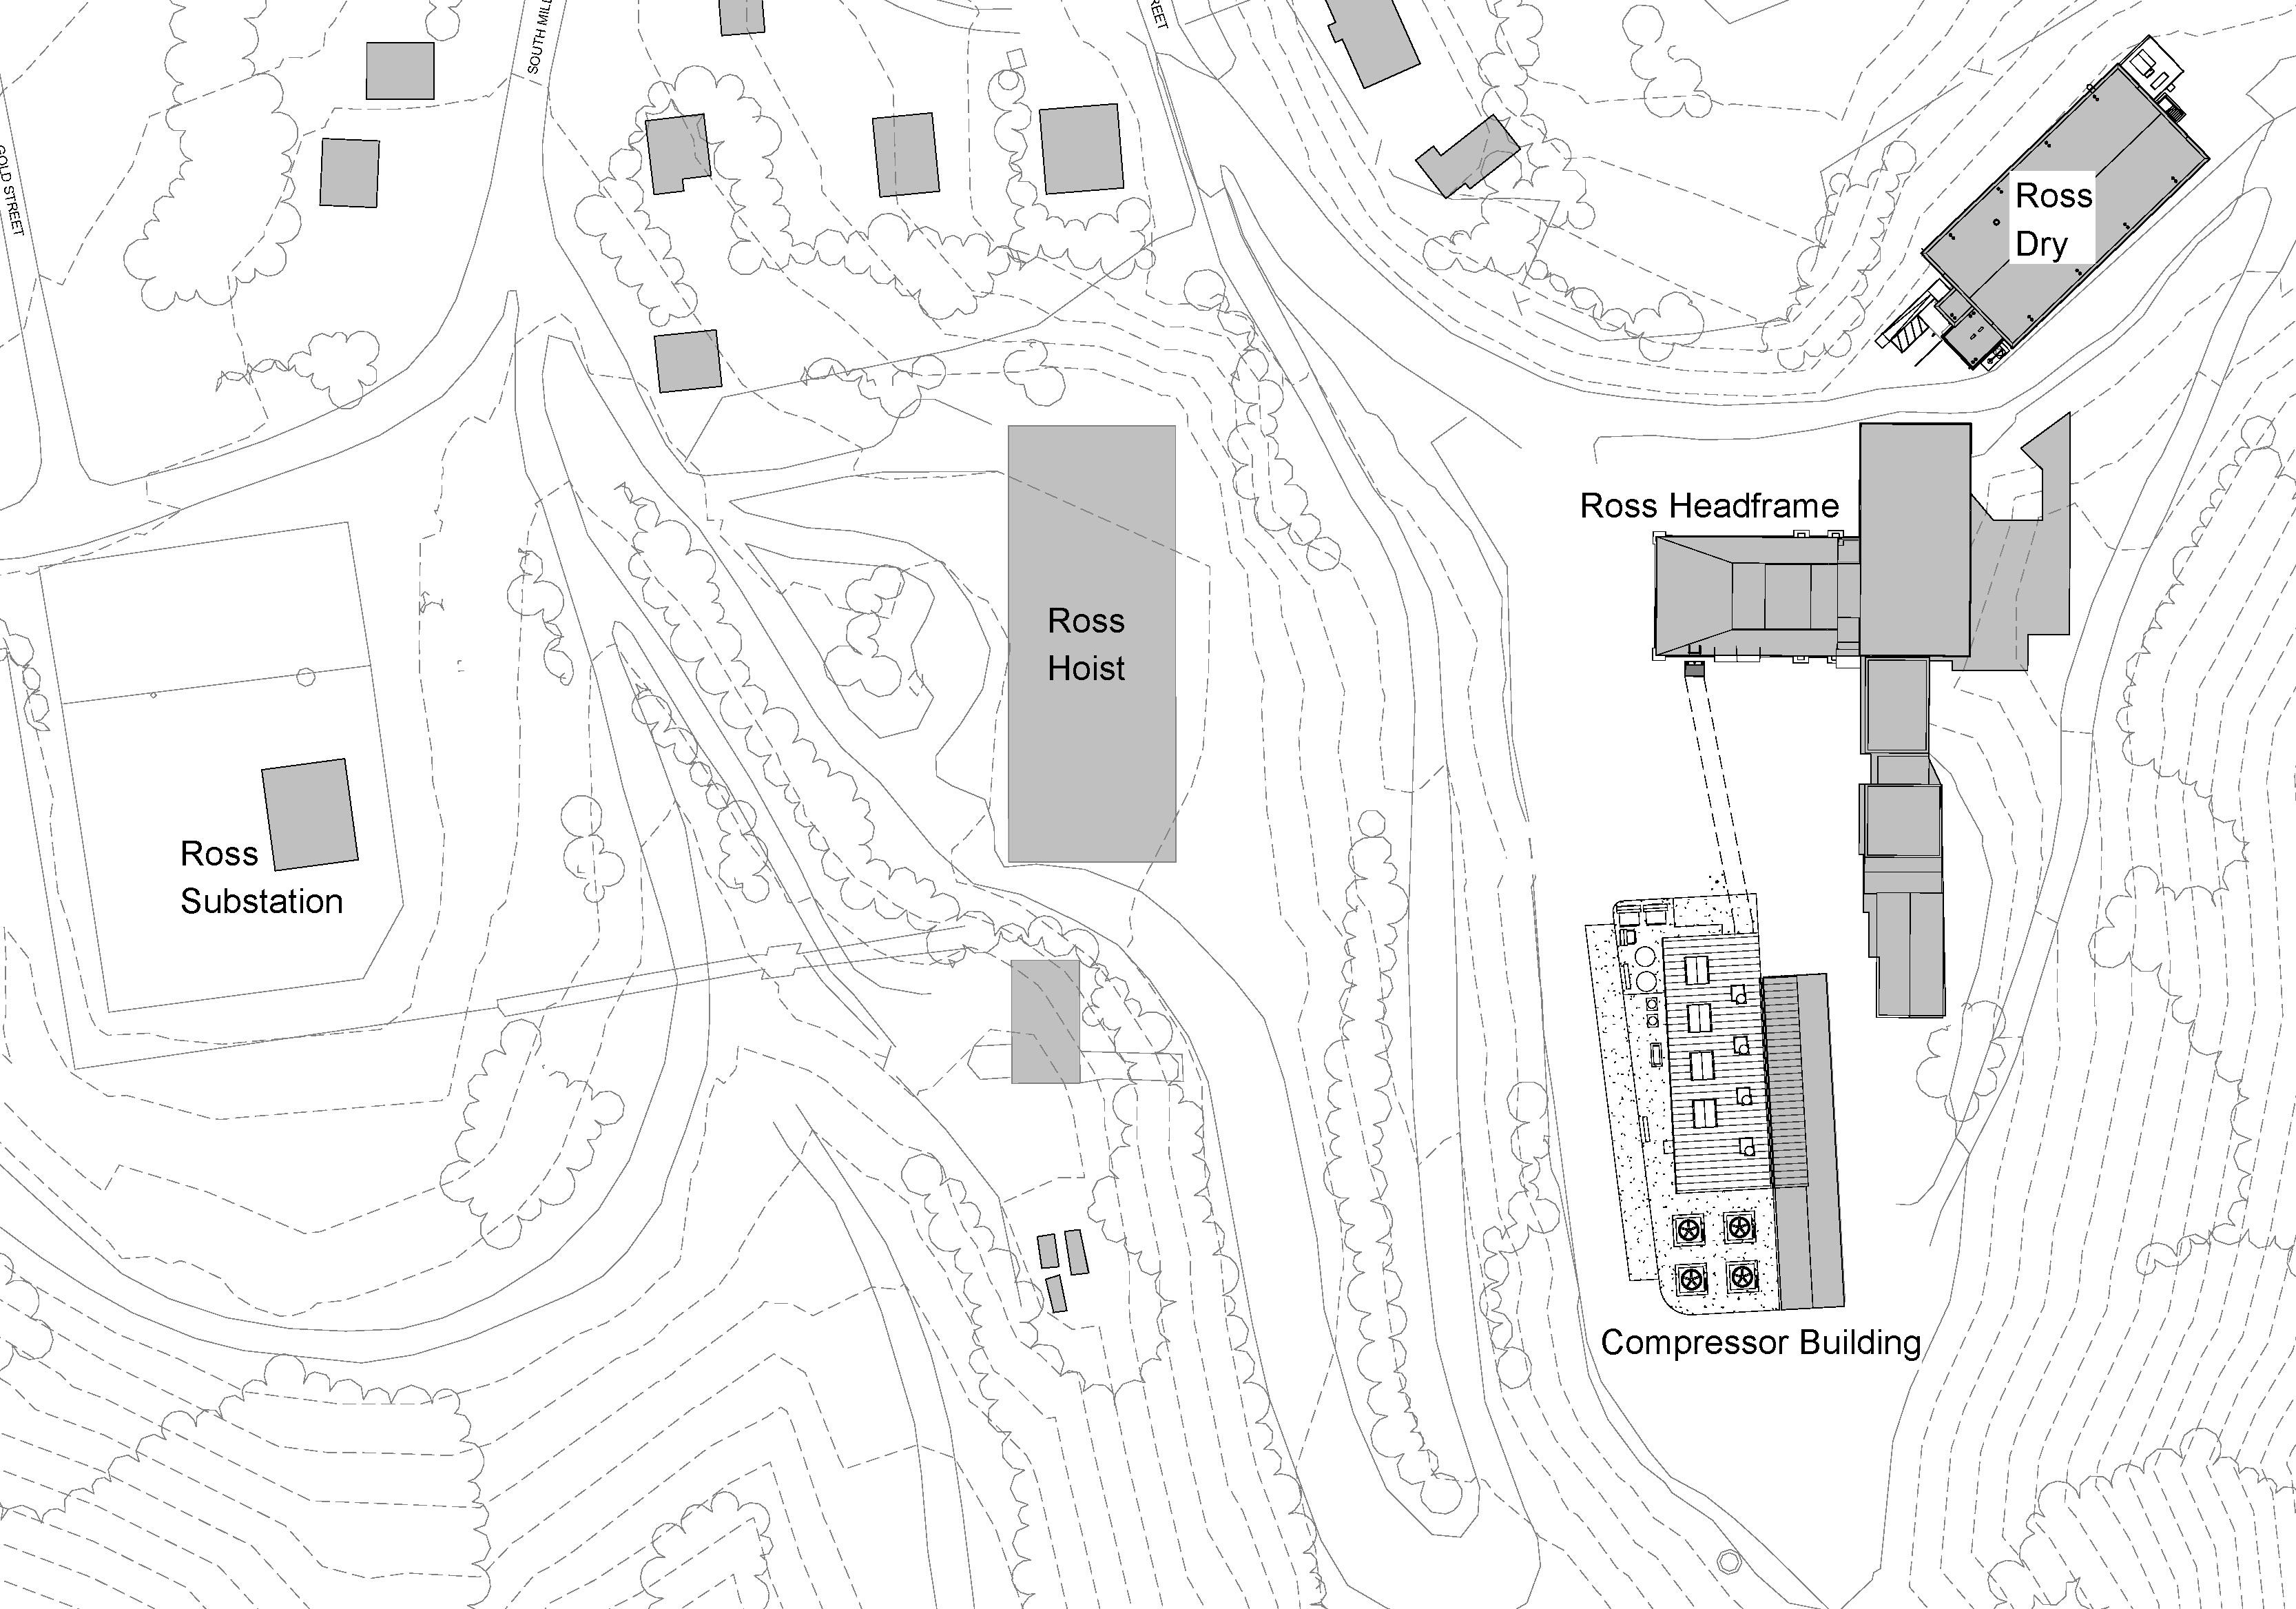
\includegraphics[width=0.8\textwidth]{ross-archit-site-plan}
\end{cdrfigure}

%%%%%%%%%%%%%%%%%%%%%%%%%%%%%%%%%%%%%%%%%%%%%%%%%%%%%%%%%%%%%%%%%%%
\section{Surface Buildings}
\label{sec:fscf-surf-facil-surface-bldg}

Surface facilities utilized for the LBNF include those necessary for safe access and egress to the underground through the Ross Shaft, as well as spaces for temporary offices (by Sanford Laboratory). Existing buildings necessary for LBNF will be rehabilitated to code-compliance and to provide for the needs of the experiment. The only new building will be to provide space for compressors use to transfer cryogens from new receiving tank on surface to the detectors underground.  The existing Ross Dry building will be modified to provide space for a surface control room and associated equipment.  Much of the text below is excerpted from the 30\% Preliminary Design Report [12] provided by Arup, USA.

A new building is planned to provide space for equipment to allow conversion of liquid argon and liquid nitrogen to gaseous form and compression of these gasses for delivery through the shaft to the underground where they are returned to liquid form as described later in this PDR in Chapter 4. \fixme{fix} The location of this building was selected based on proximity to the shaft and truck accessibility, as thousands of truckloads of argon are required to fill the detectors underground.

In addition to housing nitrogen compressors inside the building, concrete slabs are provided around the building to allow for installation of argon and nitrogen receiving dewars for truck unloading, vaporizers to boil the liquids into gas, and electrical transformer to supply power to the (4) 1,500 Hp compressors, a standby generator, and cooling towers to reject heat generated through compression.  All equipment except the cooling towers is provided by the Cryogenics Infrastructure Project. The architectural layout of this building and surrounding equipment is provided in Figure~\ref{fig:compressor-bldg}.

\begin{cdrfigure}[Architectural layout of LBNF Cryogenics Compressor Building]{compressor-bldg}{Architectural layout of LBNF Cryogenics Compressor Building}
%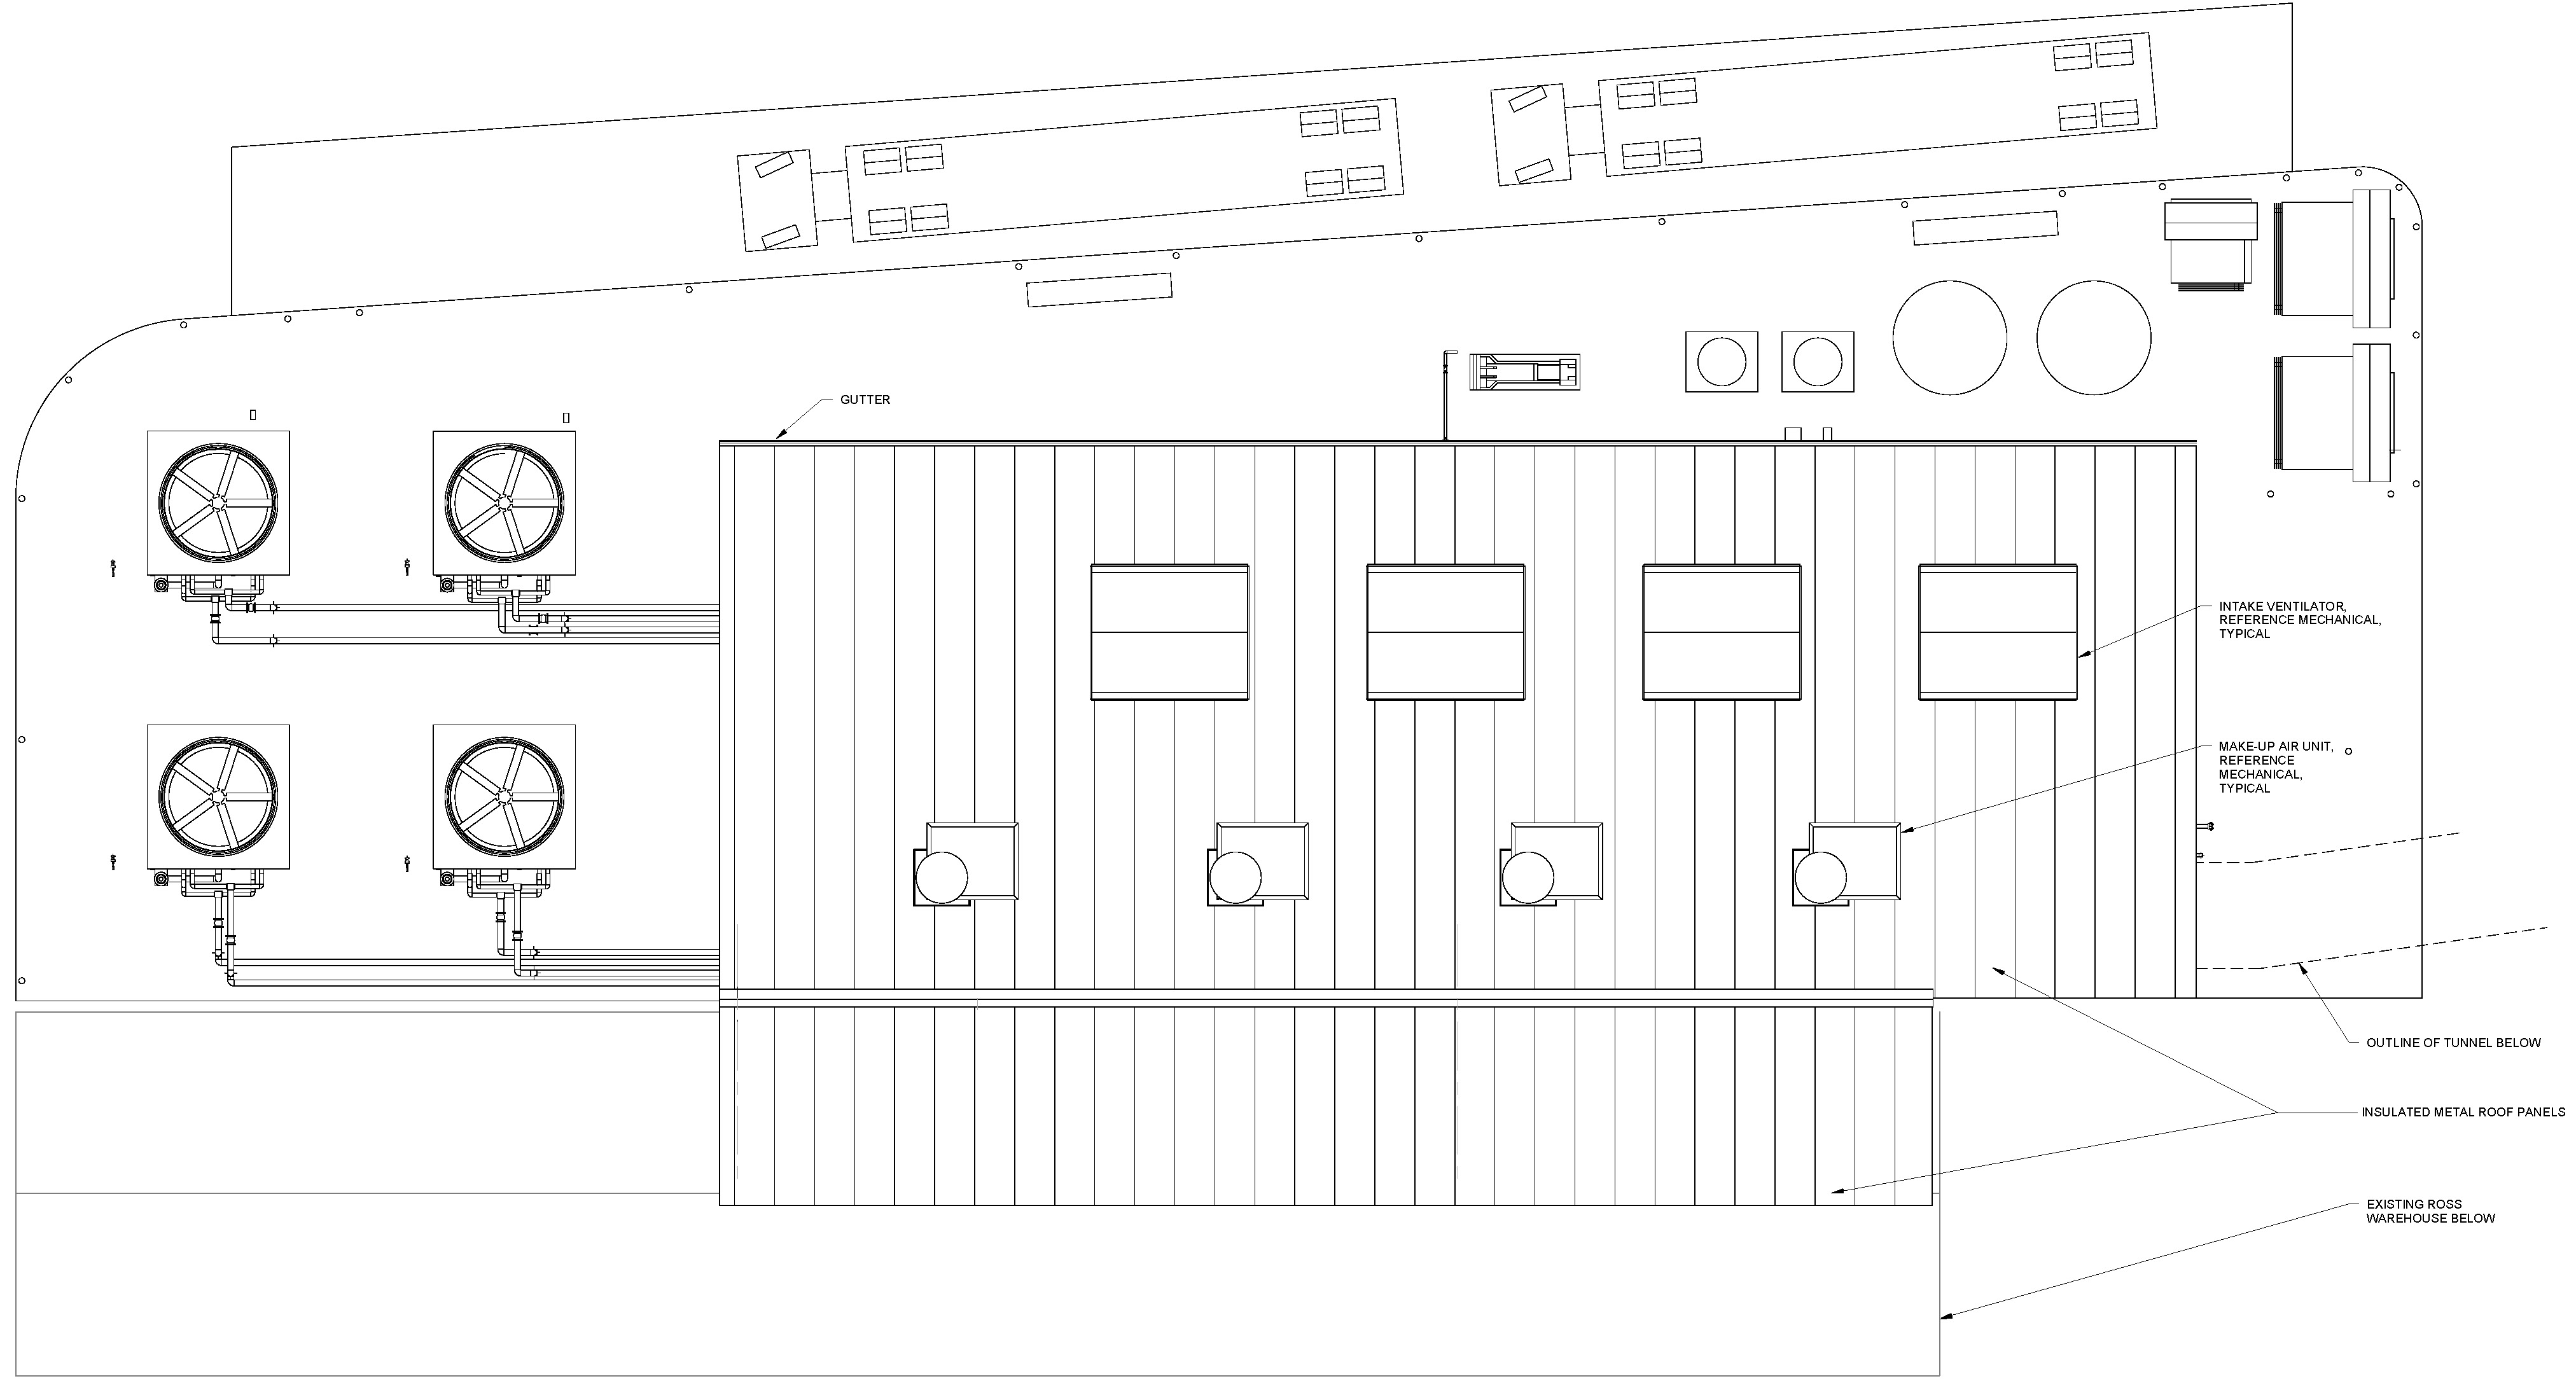
\includegraphics[width=0.8\textwidth]{compressor-bldg}
\end{cdrfigure}


%%%%%%%%%%%%%%%%%%%%%%%%%%%%%%%%%%
\subsection{Ross Dry}
\label{sec:fscf-surf-facil-surface-bldg-rossdry}

The Ross Dry building is in use by the Sanford Laboratory to provide office and meeting space in addition to men's and women's dry facilities. A portion of an existing meeting space within this building will be modified to allow the installation of a control room for both facility and experiment control.

The exterior of the Ross Dry is shown in Figure~\ref{fig:ross-dry-ext}.  The location of the new command and control center is shown in Figure~\ref{fig:cmd-control-center}.

\begin{cdrfigure}[Photo of Ross Dry exterior]{ross-dry-ext}{Photo of Ross Dry exterior (HDR)}
%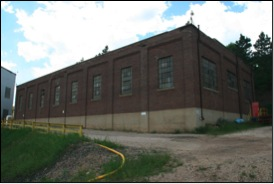
\includegraphics[width=0.8\textwidth]{ross-dry-ext}
\end{cdrfigure}

\begin{cdrfigure}[Location of new Command and Control Center]{cmd-control-center}{Location of new Command and Control Center (Sanford Lab)}
%\includegraphics[width=0.8\textwidth]{cmd-control-center}
\end{cdrfigure}

%%%%%%%%%%%%%%%%%%%%%%%%%%%%%%%%%%
\subsection{Ross Headframe and Hoist Buildings}
\label{sec:fscf-surf-facil-surface-bldg-rosshead}

The headframe and hoist buildings at the Ross Campus provide services for LBNF use. The Ross Headframe Building will be the main entry point for construction activities as well as the ongoing operations and maintenance functions. Gas pipe from the LBNF Cryogenics Compressor Building will pass through this building to get to the shaft.  

%%%%%%%%%%%%%%%%%%%%%%%%%%%%%%%%%%
\subsection{Ross Crusher Building}
\label{sec:fscf-surf-facil-surface-bldg-rosscrusher}

The existing Ross Crusher Building is a high bay space that contains rock crushing equipment that will be used for construction operations. The exterior of the building will be repaired to create a warm, usable shell. The upgrade of the existing crusher equipment is part of the waste rock handling work scope and not part of the building rehabilitation.

%%%%%%%%%%%%%%%%%%%%%%%%%%%%%%%%%%%%%%%%%%%%%%%%%%%%%%%%%%%%%%%%%%%
\section{New Surface Infrastructure}
\label{sec:fscf-surf-facil-surface-new}

Surface infrastructure includes surface structures such as retaining walls and parking lots, as well as utilities to service both buildings and underground areas. Existing infrastructure requires both rehabilitation as well as upgrading to meet code requirements and LBNF needs. The experiment needs were documented in the requirements found in LBNF Requirements Document [13] and combined with facility needs for the design detailed in the Arup 30\% Preliminary Design Report.

No new roads or parking lots are required for LBNF at the Sanford Laboratory.  The Ross Complex site will require minor demolition of power lines and a fire hydrant that are no longer used to provide adequate accessibility for truck traffic to the new Cryogenics Compressor Building.  An existing space will be designated for handicap parking adjacent to the Ross Dry Building.  Additional road work is required for truck transportation of waste rock, as described in the waste rock handling section.

